\documentclass[journal,12pt,twocolumn]{IEEEtran}
%

\usepackage{setspace}
\usepackage{gensymb}
\singlespacing

\usepackage{amsmath}
\usepackage{amsthm}
\usepackage{txfonts}
\usepackage{cite}
\usepackage{enumitem}
\usepackage{mathtools}
\usepackage{listings}
    \usepackage{color}                                            %%
    \usepackage{array}                                            %%
    \usepackage{longtable}                                        %%
    \usepackage{calc}                                             %%
    \usepackage{multirow}                                         %%
    \usepackage{hhline}                                           %%
    \usepackage{ifthen}                                           %%
  %optionally (for landscape tables embedded in another document): %%
    \usepackage{lscape}     
\usepackage{multicol}
\usepackage{chngcntr}
\renewcommand\thesection{\arabic{section}}
\renewcommand\thesubsection{\thesection.\arabic{subsection}}
\renewcommand\thesubsubsection{\thesubsection.\arabic{subsubsection}}

% correct bad hyphenation here
\hyphenation{op-tical net-works semi-conduc-tor}
\def\inputGnumericTable{}                                 %%

\lstset{
%language=C,
frame=single, 
breaklines=true,
columns=fullflexible
}

\begin{document}
%


\newtheorem{theorem}{Theorem}[section]
\newtheorem{problem}{Problem}
\newtheorem{proposition}{Proposition}[section]
\newtheorem{lemma}{Lemma}[section]
\newtheorem{corollary}[theorem]{Corollary}
\newtheorem{example}{Example}[section]
\newtheorem{definition}[problem]{Definition}
\newcommand{\BEQA}{\begin{eqnarray}}
\newcommand{\EEQA}{\end{eqnarray}}
\newcommand{\define}{\stackrel{\triangle}{=}}
\bibliographystyle{IEEEtran}
\providecommand{\mbf}{\mathbf}
\providecommand{\pr}[1]{\ensuremath{\Pr\left(#1\right)}}
\providecommand{\qfunc}[1]{\ensuremath{Q\left(#1\right)}}
\providecommand{\sbrak}[1]{\ensuremath{{}\left[#1\right]}}
\providecommand{\lsbrak}[1]{\ensuremath{{}\left[#1\right.}}
\providecommand{\rsbrak}[1]{\ensuremath{{}\left.#1\right]}}
\providecommand{\brak}[1]{\ensuremath{\left(#1\right)}}
\providecommand{\lbrak}[1]{\ensuremath{\left(#1\right.}}
\providecommand{\rbrak}[1]{\ensuremath{\left.#1\right)}}
\providecommand{\cbrak}[1]{\ensuremath{\left\{#1\right\}}}
\providecommand{\lcbrak}[1]{\ensuremath{\left\{#1\right.}}
\providecommand{\rcbrak}[1]{\ensuremath{\left.#1\right\}}}
\theoremstyle{remark}
\newtheorem{rem}{Remark}
\newcommand{\sgn}{\mathop{\mathrm{sgn}}}
\providecommand{\abs}[1]{\lvert#1\rvert}
\providecommand{\res}[1]{\Res\displaylimits_{#1}} 
\providecommand{\norm}[1]{\lVert#1\rVert}
\providecommand{\mtx}[1]{\mathbf{#1}}
% \providecommand{\mean}[1]{E\left[ #1 \right]}
\providecommand{\fourier}{\overset{\mathcal{F}}{ \rightleftharpoons}}
\providecommand{\system}{\overset{\mathcal{H}}{ \longleftrightarrow}}
\newcommand{\solution}{\noindent \textbf{Solution: }}
\newcommand{\cosec}{\,\text{cosec}\,}
\providecommand{\dec}[2]{\ensuremath{\overset{#1}{\underset{#2}{\gtrless}}}}
\newcommand{\myvec}[1]{\ensuremath{\begin{pmatrix}#1\end{pmatrix}}}
\newcommand{\cmyvec}[1]{\ensuremath{\begin{pmatrix*}[c]#1\end{pmatrix*}}}
\newcommand{\mydet}[1]{\ensuremath{\begin{vmatrix}#1\end{vmatrix}}}
\newcommand{\proj}[2]{\textbf{proj}_{\vec{#1}}\vec{#2}}
\newcommand{\RNum}[1]{\uppercase\expandafter{\romannumeral #1\relax}}
\let\StandardTheFigure\thefigure
\let\vec\mathbf
\title{
\LARGE SM5083\\
    \LARGE Assignment Number 2 \\[0.5em]
    
    \large H.N Srikanth\par
    \large   SM21MTECH12012  \par
}
\maketitle
\renewcommand{\thefigure}{\theenumi}
\renewcommand{\thetable}{\theenumi}
\section{ chapter \RNum{3} Miscellaneous Examples \RNum{6} Q.11 }

\textbf{Show that the lines $l_1x+m_1y+n_1=0,l_2x+m_2y+n_2=0$
will be equally inclined in the opposite direction if
\[\frac{m_1}{l_1}+\frac{m_2}{l_2}=2 cosw\], where w is the angle between the axes.}\\
\textbf{Solution :}\\
\textbf{Given :}\[\frac{m_1}{l_1}+\frac{m_2}{l_2}=2 cosw\]

Here w is the angle between the axes\\
\textbf{To proove :} $l_1x+m_1y+n_1=0, l_2x+m_2y+n_2=0$
will be equally inclined in the opposite direction.
This implies magnitudes of slopes of $l_1x+m_1y+n_1=0,l_2x+m_2y+n_2=0$ are equal.\\
From given condition
\[\frac{m_1}{l_1}+\frac{m_2}{l_2}=2 cosw\]
\[\frac{m_1l_2+m_2l_1}{l_1l_2}=2 cosw\]
\[\frac{m_1l_2+m_2l_1}{m_1m_2}=2\frac{l_1l_2}{m_1m_2} cosw\]
\begin{equation}\label{eq1}
\frac{l_1}{m_1}+\frac{l_2}{m_2}=2\frac{l_1l_2}{m_1m_2} cosw
\end{equation}
let
\begin{equation}\label{eq2}
a_1=\frac{-l_1}{m_1}
\end{equation}
\begin{equation}\label{eq3}
a_2=\frac{-l_2}{m_2}
\end{equation}
Here $a_1, a_2$ are slopes of the lines in transformed axes. By substituting \eqref{eq2} and \eqref{eq3} in \eqref{eq1}\\
$a_1+a_2=-2a_1a_2cosw$\\
$a_1+a_1a_2cosw=-a_2-a_1a_2cosw$
\begin{equation}\label{eq4}
\frac{a_1sinw}{1+a_1cosw}=\frac{-a_2sinw}{1+a_2cosw}
\end{equation}
    
\eqref{eq4} shows the equivalent slopes of lines $l_1x+m_1y+n_1=0,l_2x+m_2y+n_2=0$ in cartesian axes 


\eqref{eq4} also depicts that slopes are equal and lines are in opposite direction.
\begin{figure}[!ht]
	\centering
	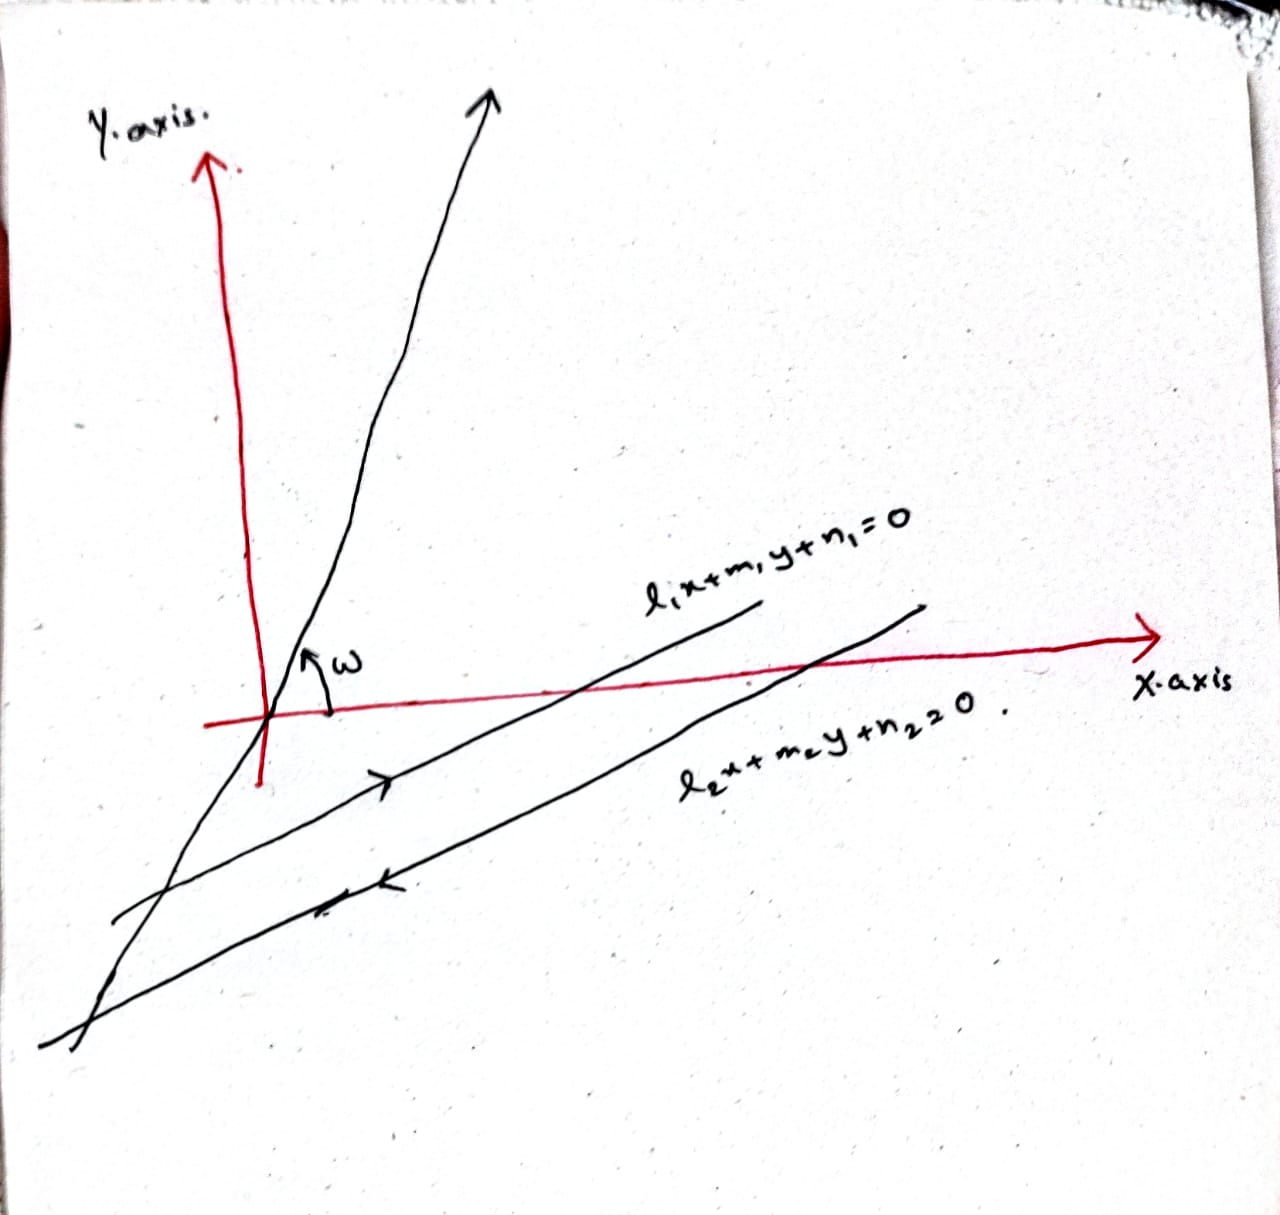
\includegraphics[width=\columnwidth]{assignment_2.jpeg}
	\caption{}
	\label{fig:assignment02}
\end{figure}

\end{document}